\section{Additional nPDF impact studies}
\label{app:nPDF_impact_appendix}

%%%%%%%%%%%%%%%%%%%%%%%%%%%%%%%%%%%%%%%%%%%%%%%%%%%%%%%%%%%%%%%%%%%%%%%%
\begin{figure*}[htbp]
	\centering
	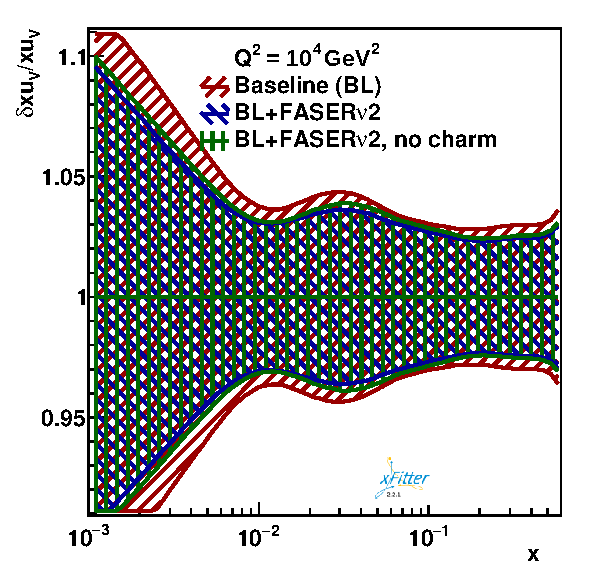
\includegraphics[width=0.32\textwidth]{plots/nuclear_fasernu2/inclusive-only_vs_inclusive+charm/statOnly_FASERv2_q2_10000_pdf_uv_ratio.pdf}
	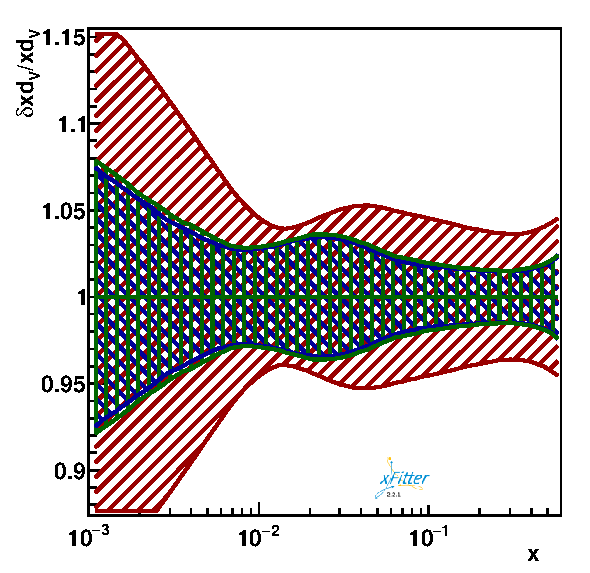
\includegraphics[width=0.32\textwidth]{plots/nuclear_fasernu2/inclusive-only_vs_inclusive+charm/statOnly_FASERv2_q2_10000_pdf_dv_ratio.pdf}
	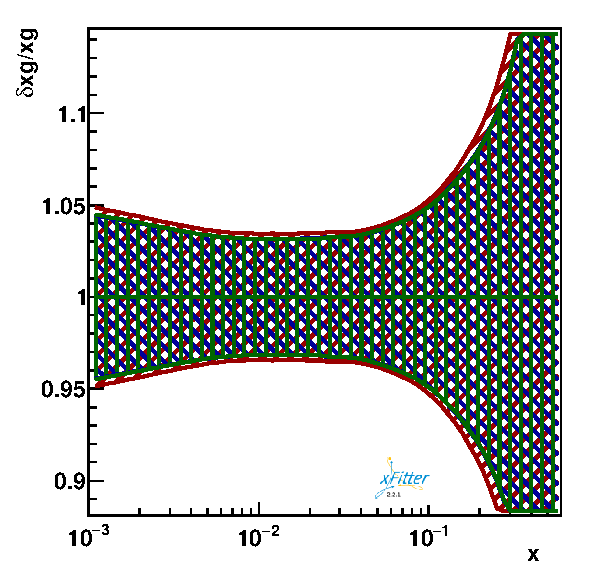
\includegraphics[width=0.32\textwidth]{plots/nuclear_fasernu2/inclusive-only_vs_inclusive+charm/statOnly_FASERv2_q2_10000_pdf_g_ratio.pdf}\\
	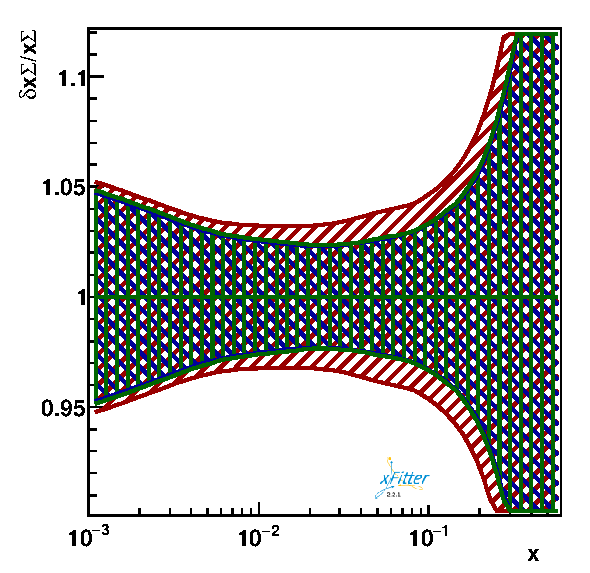
\includegraphics[width=0.32\textwidth]{plots/nuclear_fasernu2/inclusive-only_vs_inclusive+charm/statOnly_FASERv2_q2_10000_pdf_Sea_ratio.pdf}
	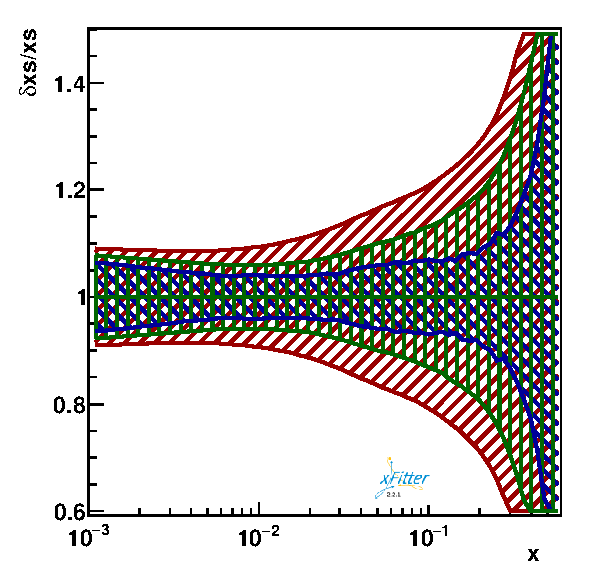
\includegraphics[width=0.32\textwidth]{plots/nuclear_fasernu2/inclusive-only_vs_inclusive+charm/statOnly_FASERv2_q2_10000_pdf_s_ratio.pdf}\\
	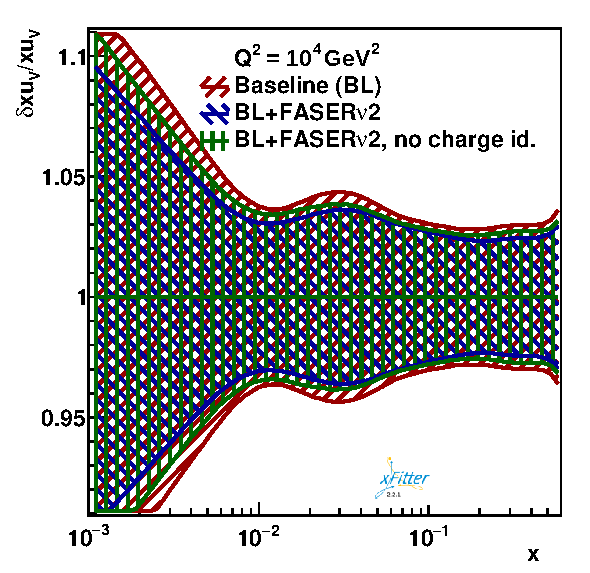
\includegraphics[width=0.32\textwidth]{plots/nuclear_fasernu2/nochargediscrimination/statOnly_FASERv2_q2_10000_pdf_uv_ratio.pdf}
	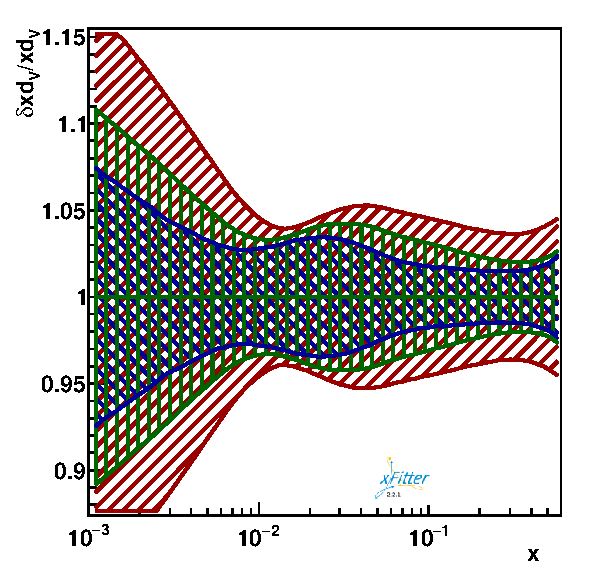
\includegraphics[width=0.32\textwidth]{plots/nuclear_fasernu2/nochargediscrimination/statOnly_FASERv2_q2_10000_pdf_dv_ratio.pdf}
	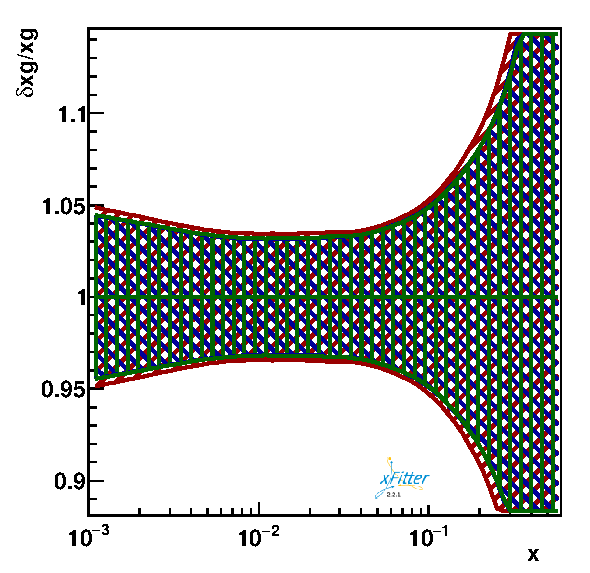
\includegraphics[width=0.32\textwidth]{plots/nuclear_fasernu2/nochargediscrimination/statOnly_FASERv2_q2_10000_pdf_g_ratio.pdf}\\
	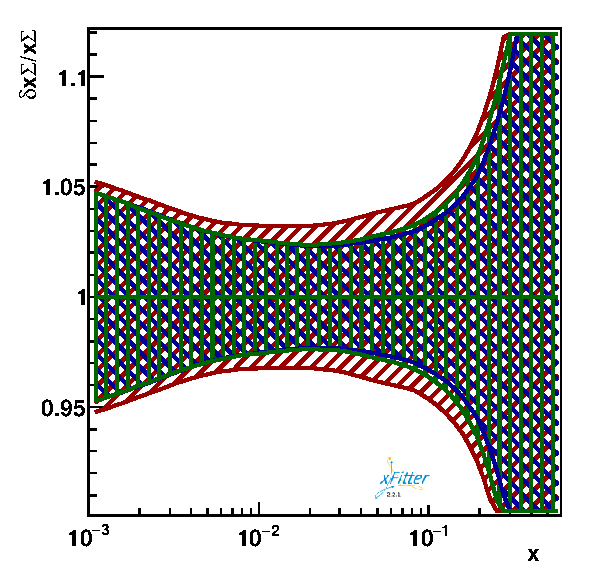
\includegraphics[width=0.32\textwidth]{plots/nuclear_fasernu2/nochargediscrimination/statOnly_FASERv2_q2_10000_pdf_Sea_ratio.pdf}
	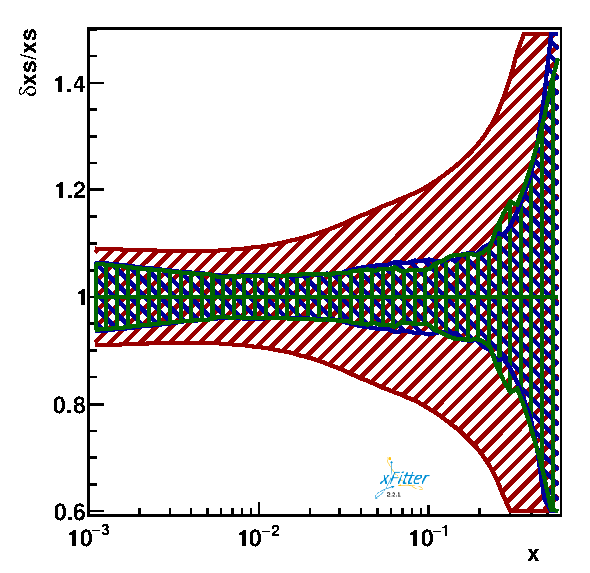
\includegraphics[width=0.32\textwidth]{plots/nuclear_fasernu2/nochargediscrimination/statOnly_FASERv2_q2_10000_pdf_s_ratio.pdf}
	\caption{Same as Fig.~\ref{fig:FASERnu2_nocharm} (upper panels)
		and  Fig.~\ref{fig:FASERnu2_nochargeID} (bottom panels) in the case of EPPS21.
	}
	\label{fig:EPPS21_nochargeID}
\end{figure*}
%%%%%%%%%%%%%%%%%%%%%%%%%%%%%%%%%%%%%%%%%%%%%%%%%%%%%%%%%%%%%%%%%%%%%%%%

The impact of FPF structure function measurements on the
EPPS21 nuclear PDF determination has been studied in Sect.~\ref{sec:nuclearPDFs}.
%
Here we provide additional results from this study, and specifically quantify the impact
that removing charm-tagged structure functions and flavour-charge
identification capabilities would have on the projected results.
%
Fig.~\ref{fig:EPPS21_nochargeID} displays
the analogous comparisons as in Figs.~\ref{fig:FASERnu2_nocharm}
and~\ref{fig:FASERnu2_nochargeID} in the case of EPPS21.
%
In both cases, results are consistent with the proton PDF profiling analysis.

First of all, charm-tagged events are essential to achieve the best
sensitivity to the strange PDF, while they have a vanishing impact on the
other PDF combinations.
%
Second, not being able to identify the charge of the outgoing final-state lepton
does not markedly affect  the baseline results, with the possible exception
of the down valence quark PDF.
%
As discussed in Sect.~\ref{sec:nudis_revisited}, for a non-isoscalar target
such as tungsten, with $Z=74$ and $A-Z=110$, event rates with neutrino projectiles
will differ from those arising from antineutrino scattering, introducing
additional information as compared to an isoscalar target in terms of PDF sensitivity.


